\documentclass[main.tex]{subfiles}

\begin{document}

\section{Classical Learning Theory}

\section{Boolean Fourier Analysis}

\section{Randomized Linear Algebra}

\section{Algorithms for solving linear systems of equations}

One such application of Phase Estimation (Section \ref{phase_estimation}) is with respect to solving linear systems of equations. This is the so-called HHL algorithm \cite{lloyd2010quantum}.

The general problem statement of a linear system is if we are given matrix $A$ and unit vector $\vec{b}$, then find $\vec{x}$ satisfying, $A\vec{x} = \vec{b}$. 

However, assume that instead of solving for $x$ itself, we instead solve for an expectation value $x^T M x$ for some linear operator $M$. Hence, one can show that our algorithm has a runtime bound of $O(\log(N)\kappa ^{2})$, if we can further assume that the linear system is sparse and has a low condition number $\kappa$.

So, assume that $A$ in our linear system is an $N \times N$ Hermitian matrix. Notice that this is an "unrestrictive" constraint on $A$ because we can always take non-Hermitian matrix $A'$ and linear system $A' \vec{x} = \vec{b}$ and instead solve $\begin{bmatrix}
	0 && A' \\ A'^\dag && 0
\end{bmatrix} \begin{bmatrix} 0 \\ x \end{bmatrix} = \begin{bmatrix} b \\ 0 \end{bmatrix}$. Hence, we we will assume that $A$ is Hermitian from here on. 

Recall that because $A$ is hermitian $\implies$ we can perform quantum phase estimation using $e^{-iAt}$ as the unitary transformation. This can be done efficiently if $A$ is sparse.

So, we first prepare $\ket{b}$ (the representation of $\vec{b}$). We assume that this can be done efficiently or that $\ket{b}$ is supplied as an input.

Denote by $\ket{\psi_j}$ the eigenvectors of $A$ with associated eigenvalues $\lambda_j$. Hence, we can express $\ket{b}$ as $\ket{b} = \sum_j \beta_j \ket{\psi_j}$.  So, we initialize a first register to state $\sum_j \beta_j \ket{\psi_j}$ and second register to state $\ket{0}$ . After applying phase estimation, we then have the joint state $\sum_j \beta_j \ket{\psi_j} \ket{\widetilde{\lambda}_j}$, where $\widetilde{\lambda}_j$ is an approximation of $\lambda_j$. We'll assume that this approximation is perfect from here on. 

Next we add an ancilla qubit and perform a rotation conditional on the first register while now holds $\ket{\lambda_j}$. The rotation transforms the system to

\begin{align*}
\sum_j \beta_j \ket{\psi_j} \ket{\lambda_j} \Big(\sqrt{1-\frac{C^2}{\lambda_j^2}}\ket{0} + \frac{C}{\lambda_j}\ket{1}\Big)
\end{align*}

for some small constant $C \in \RR$ that is $O(1/\kappa)$.

Hence, we can undo phase estimation to restore the second register to $\ket{0}$.

Now, if we measure the ancillary qubit in the computational basis, we'll evidently collapse the state to $\ket{1}$ with some probability. We'd then have

\begin{align*}
	\sum_j \frac{C}{\lambda_j} \beta_j \ket{\psi_j} \ket{\lambda_j}\ket{1} = C (A^{-1} \ket{b})
\end{align*}

In particular, the probability of getting this result is 

\begin{align*} 
	p(-1) &= \Bigg(\sum_j \beta_j \bra{\psi_j} \bra{\lambda_j} \Big(\sqrt{1-\frac{C^2}{\lambda_j^2}}\bra{0} + \frac{C}{\lambda_j}\bra{1}\Big) \Bigg)\ket{1}\bra{1} \Bigg(\sum_j \beta_j \ket{\psi_j} \ket{\lambda_j} \Big(\sqrt{1-\frac{C^2}{\lambda_j^2}}\ket{0} + \frac{C}{\lambda_j}\ket{1}\Big)\Bigg) \\
	&= \sum_j \beta_j \bra{\psi_j} \bra{\lambda_j} \Big(\sqrt{1-\frac{C^2}{\lambda_j^2}}\bra{0} + \frac{C}{\lambda_j}\bra{1}\Big) \ket{1}\bra{1} \beta_j \ket{\psi_j} \ket{\lambda_j} \Big(\sqrt{1-\frac{C^2}{\lambda_j^2}}\ket{0} + \frac{C}{\lambda_j}\ket{1}\Big) \\
	&= \sum_j \beta_j \bra{\psi_j} \bra{\lambda_j} \frac{C}{\lambda_j}\bra{1}\ket{1}\bra{1} \beta_j \ket{\psi_j} \ket{\lambda_j} \frac{C}{\lambda_j}\ket{1} \\
	&= \sum_j \beta_j^2 \frac{C^2}{\lambda_j^2} \\
	&= \| A^{-1} \ket{b} \|^2 C^2 = O(1/\kappa^4)
\end{align*} 

Finally, we can make a measurement $M$ whose expectation value $\bra{x}M\ket{x}$ corresponds to the feature of $x$ we wish to evaluate. 

\section{Supervised learning with quantum feature Hilbert spaces}
\cite{havlicek2018supervised}

\subsection{Prelude}

We are given data from a training set $T$ and a test set $S$ of a subset $\Omega \subset \RR^d$. We assume that $S$ and $T$ are drawn from the same input space $X$. Furthermore, there exists output space $Y = \{ -1, +1 \} $ and a distribution $D$ on $X \times Y$.

Now, suppose we have a labelling $m: T \cup S \rightarrow Y$.  Our goal is to use this information to find some approximation function $\tilde{f} : X \rightarrow Y$ that minimizes estimation error for function class $F$. In other words, let true risk for function $f$ be defined as

\begin{align*}
R^{true}(f) = P_{X, Y \sim D}(f(X) \neq Y)	
\end{align*}

Then, estimation error is the difference in true risk between $\tilde{f}$ and optimal choice $f^* = \inf_{f \in F}R^{true}(f)$.

One classical method is using so-called Support Vector Machines (SVM), which construct a separating hyperplane such that the distance to the nearest training observation (minimum margin) is maximized. Much of the popularity of SVMs can be attributed to its association with the "kernel trick" which maps the data to a higher dimensional space so that it is separable or approximately separable.

Here, we suppose that the data is given classically and we seek to show that, in some cases, we can obtain a quantum advantage by either generating the separating hyperplane in quantum feature space or simply estimating the kernel function.

\subsection{Feature Map}

Consider the feature vector kernel $K(x, z) = | \bra{\Phi(x)}\ket{\Phi(z)} |^2$

\subsection{Quantum Variational Classification}

\subsection{Quantum Kernel Estimation}

\subsection{Non-Trivial Feature Map with Entanglement}

\subsection{Geometric Analysis of Candidate Feature Maps}

\subsection{Experimental Simulation of Candidate Feature Maps}

%\section{Density Matrix Exponentiation Algorithms}
%\url{https://www.nature.com/articles/nphys3029}
%
%\section{Review of Quantum Machine Learning}
%\url{https://www.nature.com/articles/nature23474}
%
%\section{Learnability of Quantum States}
%\begin{enumerate}
%\item \url{https://arxiv.org/abs/quant-ph/0608142}
%\item \url{https://arxiv.org/abs/1711.01053}
%\item \url{https://arxiv.org/abs/1801.05721}
%\end{enumerate}


\section{Singular Value Transformation using Quantum-Inspired Length-Square Sampling Methods}

As we've seen, most well-known QML algorithms convert input quantum states to a desired output state or value. Thus, they do not provide a routine to get necessary copies of these input states (a state preparation routine) and a strategy to extract information from an output state. Both are essential to making the algorithm useful.

\begin{itemize}
    %\item HHL algorithm: application of phase estimation and Hamiltonian simulation to solve linear system.
    \item We can compute $A^+ \ket{b} = \ket{x_{LS}}$ in $\tilde{O}(log(N)(s^3\kappa^6)/ \epsilon)$ time (query complexity)
    \item Uses a quantum algorithm based on phase estimation and Hamiltonian simulation
    \item Assumption: $A$ is sparse with low condition number $\kappa$. Hamiltonian ($\hat{H}$) simulation is efficient when $\hat{H}$ is sparse. No low-rank assumptions are necessary.
    \item "Key" assumption: the quantum state $\ket{b}$ can be prepared efficiently.	
    \item What happens if we assume low rank?
\end{itemize}

\begin{itemize}
\item In general, quantum machine learning algorithms convert quantum input states to the desired quantum output states. 
\item In practice, data is initially stored classically and the algorithm's output must be accessed classically as well.
\item Today's focus: A practical way to make comparisons between classical and quantum algorithms is to analyze classical algorithms under $\ell^2$ sampling conditions
\item Tang: linear algebra problems in low-dimensional spaces (say constant or polylogarithmic) likely can be solved "efficiently" under these conditions
\item Many of the initial practical applications of quantum machine learning were to problems of this type (e.g. Quantum Recommendation Systems - Kerendis, Prakash, 2016)
\end{itemize}

\begin{itemize}
\item How can we compare the speed of quantum algorithms with quantum input and quantum output to classical algorithms with classical input and classical output? 
\item Quantum machine learning algorithms can be exponentially faster than the best standard classical algorithms for similar tasks, but quantum algorithms get help through input state preparation. 
\item Want a practical classical model that helps its algorithms offer similar guarantees to quantum algorithms, while still ensuring that they can be run in nearly all circumstances one would run the quantum algorithm. 
\item Solution (Tang): compare quantum algorithms with quantum state preparation to classical algorithms with sample and query access to input.	
\end{itemize}

\subsubsection{Definitions}

\begin{definition}
We have "query access" to $x \in \CC^n$ if, given $i \in [n]$, we can efficiently compute $x_i$. We say that $x \in \mathcal{Q}$.
\end{definition}
\begin{definition} We have sample \textbf{and} query access to $x \in \CC^n$ if 

\begin{enumerate}
\item We have query access to $x$ i.e. $x\in \mathcal{Q}$ ($\implies$ $\mathcal{SQ} \subset \mathcal{Q}$)
\item can produce independent random samples $i \in [n]$ where we sample $i$ with probability $|x_i|^2/\|x\|^2∣$ and can query for $\|x\|$.
\end{enumerate}
We say that $x \in \mathcal{SQ}$. 
\end{definition}
\begin{definition} For $A \in \CC^{m\times n}$, $A \in \mathcal{SQ}$ (abuse) if

\begin{enumerate}
\item $A_i \in \mathcal{SQ}$ where $A_i$ is the $i$th row of $A$
\item $\tilde{A} \in \mathcal{SQ}$ for $\tilde{A}$ the vector of row norms (so $\tilde{A}_i = \|A_i\|$).	
\end{enumerate}
\end{definition}


\begin{example}
Say we have the vector $\vec{x} = (2, 0, 1, 3)$ and $\vec{x} \in \mathcal{SQ}$. Consider the following binary tree data structure.

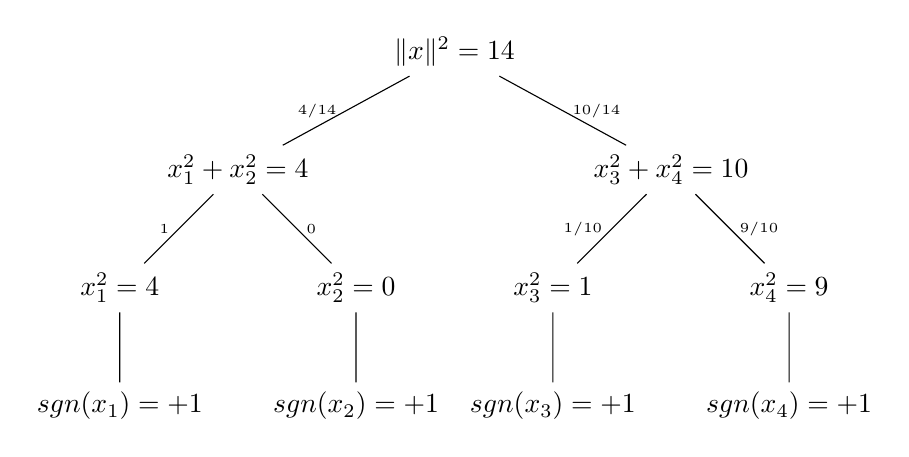
\begin{tikzpicture}[level distance=1.5cm,
  level 1/.style={sibling distance=5.5cm},
  level 2/.style={sibling distance=3cm}, 
  level 3/.style={sibling distance=3cm}]
  \node (1){$\| x \|^2 = 14$}
    child {node {$x_1^2 + x_2^2 = 4$}
      child {node {$x_1^2 = 4$}
      	child {node {$\text{sgn}(x_1) = +1$}}
      	edge from parent node [left] {\tiny $1$}
      }
      child {node {$x_2^2 = 0$} 
      	child {node {$\text{sgn}(x_2) = +1$}}
      	edge from parent node [right] {\tiny $0$}
      }
      edge from parent node [left] {\tiny $4/14$}
    }
    child {node(2) {$x_3^2 + x_4^2 = 10$}
    	child {node {$x_3^2 = 1$}
    		child {node {$\text{sgn}(x_3) = +1$}}
    		edge from parent node [left] {\tiny $1/10$}
    	}
      child {node(3) {$x_4^2 = 9$} 
      		child {node {$\text{sgn}(x_4) = +1$}}
      		edge from parent node [right] {\tiny $9/10$}
      } 
      edge from parent node [right] {\tiny $10/14$}
    };
\end{tikzpicture}
\end{example}


\subsubsection{Low-Rank Estimation}

\begin{itemize}
\item For $A \in \CC^{m\times n}$, given $A \in \mathcal{SQ}$ and some threshold $k$, we can output a description of a low-rank approximation of $A$ with $\text{poly}(k)$ queries.
\item Specifically, we output two matrices $S,\hat{U}\in \mathcal{SQ}$ where $S \in \CC^{\ell \times n}$, $\hat{U} \in \CC^{\ell \times k}$ ($\ell = \text{poly}(k,\frac{1}{\epsilon}$)), and this implicitly describes the low-rank approximation to $A$, $D := A(S^\dagger\hat{U})(S^\dagger\hat{U})^\dag$ ($\implies$ rank $D \leq k$).

\item This matrix satisfies the following low-rank guarantee with probability $\geq 1-\delta$: for $\sigma := \sqrt{2/k}\|A\|_F$, and $A_{\sigma} := \sum_{\sigma_i \geq \sigma} \sigma_iu_iv_i^\dag$ (using SVD), 
$$\|A - D\|_F^2 \leq \|A - A_\sigma\|_F^2 + \epsilon^2\|A\|_F^2$$
\item Note the $\|A - A_\sigma\|_F^2$ term. This says that our guarantee is weak if $A$ has no large singular values. 
\item Quantum analog: phase estimation
\end{itemize}


$$
\begin{bmatrix}
\\
\cdots A \cdots 
\\
\\	
\end{bmatrix}
\begin{bmatrix}
\\
S^\dag
\\
\\	
\end{bmatrix}
\begin{bmatrix}
\hat{U}
\end{bmatrix}
\begin{bmatrix}
\hat{U^\dag}
\end{bmatrix}
\begin{bmatrix}
\cdots S \cdots
\end{bmatrix}
$$

\subsubsection{Trace Inner Product Estimation}

\begin{itemize}
	\item For $x, y \in \CC^n$, if we are given that $x \in \mathcal{SQ}$ and $y \in \mathcal{Q}$, then we can estimate $\< x, y\>$ with probability $\geq 1 - \delta$ and error $\epsilon \|x\|\|y\|$ 
	\item Quantum analog: SWAP test
\end{itemize}
\begin{figure}
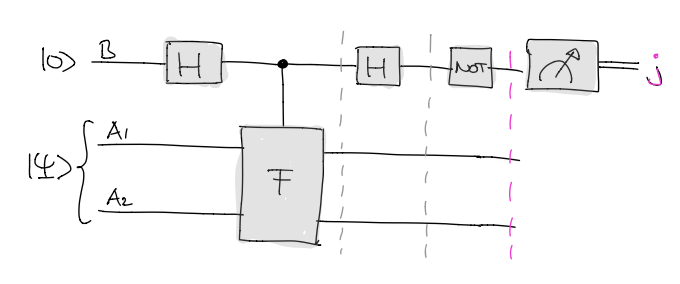
\includegraphics[width= 0.5\linewidth]{images/swap_test.png}	
\end{figure}

\begin{fact} For $\{X_{i,j}\}$ i.i.d random variables with mean $\mu$ and variance $\sigma^2$, let 

$$Y := \underset{j \in [\log 1/\delta]}{\operatorname{median}}\;\underset{i \in [1/\epsilon^2]}{\operatorname{mean}}\;X_{i,j}$$

Then $\vert Y - \mu\vert \leq \epsilon\sigma$ with probability $\geq 1-\delta$, using only $O(\frac{1}{\epsilon^2}\log\frac{1}{\delta})$ samples.
\end{fact}

\begin{itemize}
	\item In words: We may create a mean estimator from $1/\epsilon^2$ samples of $X$. We compute the median of $\log 1/\delta$ such estimators
	\item Catoni (2012) shows that Chebyshev's inequality is the best guarantee one can provide when considering pure empirical mean estimators for an unknown distribution (and finite $\mu, \sigma$)
	\item "Median of means" provides an exponential improvement in probability of success ($1 - \delta$) guarantee
\end{itemize}

\begin{corollary} For $x,y \in\CC^n$, given $x \in \mathcal{SQ}$ and $y \in \mathcal{Q}$, we can estimate $\langle x,y\rangle$ to $\epsilon\|x\|\|y\|$ error with probability $\geq 1-\delta$ with query complexity $O(\frac{1}{\epsilon^2}\log\frac{1}{\delta})$
\end{corollary}
\begin{proof}Sample an \textbf{index} $s$ from $x$. Then, define $Z := x_s y_s\frac{\|y\|^2}{|y_s|^2}$. Apply the Fact with $X_{i,j}$ being independent samples $Z$.
\end{proof}	

\subsubsection{Least-Square Sample Generation}

\begin{itemize}
	\item For $V \in \CC^{n\times k}, w \in \CC^k$, given $V^\dagger \in \mathcal{SQ}$ (\textit{column}-wise sampling of $V$) and $w \in \mathcal{Q}$, we can simulate $Vw \in \mathcal{SQ}$ with $\text{poly}(k)$ queries
	\item In words: if we can least-square sample the columns of matrix $V$ and query the entries of vector $w$, then
\begin{enumerate}
\item  We can query entries of their multiplication ($Vw$) 
\item We can least-square sample from a distribution that emulates their multiplication	
\end{enumerate}

\item Hence, as long as $k \ll n$, we can perform  each using a number of steps polynomial in the number of columns of $V$. 

\end{itemize}

\begin{definition}
Rejection sampling
\end{definition}
\begin{algorithm}
Input: Samples from distribution $P$

Output: Samples from distribution $Q$
\begin{itemize}
\item Sample $s$ from $P$
\item Compute $r_s = \frac{1}{N}\frac{Q(s)}{P(s)}$, for fixed constant $N$
\item Output $s$ with probability $r_s$ and restart otherwise
\end{itemize}
\end{algorithm}

\begin{fact}
Fact. If $r_i \leq 1, \forall i$, then the above procedure is well-defined and outputs a sample from $Q$ in $N$ iterations in expectation.	
\end{fact}


\begin{proposition}
	 For $V \in \RR^{n\times k}$ and $w \in \RR^k$, given $V^\dag \in \mathcal{SQ}$ and $w \in \mathcal{Q}$, we can simulate $Vw \in \mathcal{SQ}$ with expected query complexity $\tilde{O}((\frac{1}{\epsilon^2}\log\frac{1}{\delta}))$

We can compute entries $(Vw)_i$ with $O(k)$ queries.

We can sample using rejection sampling:

\begin{itemize}
\item $P$ is the distribution formed by sampling from $V_{(\cdot, j)}$.
  
\item $Q$ is the target $Vw$.
\item Hence, compute $r_s$ to be a constant factor of $Q / P$
\end{itemize}

$$r_i = \frac{\|w^T V_{\cdot, i}\|^2}{\|w\|^2\|V_{\cdot, i}\|^2}$$
\end{proposition}

\begin{itemize}
\item Notice that we can compute these $r_i$'s (in fact, despite that we cannot compute probabilities from the target distribution), and that the rejection sampling guarantee is satisfied (via Cauchy-Schwarz).

\item Since the probability of success is $\|Vw\|^2/ \| w\|^2$, it suffices to estimate the probability of success of this rejection sampling process to estimate this norm.

\item Through a Chernoff bound, we see that the average of $O(\|w\|^2(\frac{1}{\epsilon^2}\log\frac{1}{\delta}))$ "coin flips" is in $[(1-\epsilon)\|Vw\|,(1+\epsilon)\|Vw\|]$ with probability $\geq 1-\delta$.
\end{itemize}

\subsubsection{Application: Stochastic Regression}

For a low-rank matrix $A \in \RR^{m\times n}$
  and a vector $b \in \RR^n$, given $b, A \in \mathcal{SQ}$, (approximately) simulate $A^+b \in \mathcal{SQ}$.

\begin{algorithm}   	
\begin{itemize}
\item Low-rank approximation (3) gives us $S,\hat{U} \in \mathcal{SQ}$.

\item Applying thin-matrix vector (2), we get $\hat{V} \in \mathcal{SQ}$, where $\hat{V} := S^T\hat{U}$; we can show that the columns of $\hat{V}$ behave like the right singular vectors of $A$.
\item Let $\hat{U}$ have columns $\{ \hat{u}_i\}$. Hence, $\hat{V}$ has columns $\{ S \hat{u}_i \}$. Write its $i$th column as $\hat{v}_i := S\hat{u}_i$.

\item Low-rank approximation (3) also outputs the approximate singular values $\hat{\sigma}_i$ of $A$
\end{itemize}
\end{algorithm}

Now, we can write the approximate vector we wish to sample in terms of these approximations:

$$A^+b = (A^TA)^+A^Tb \approx \sum_{i=1}^k \frac{1}{\hat{\sigma}_i^2}\hat{v}_i\hat{v}_i^T A^Tb$$

\begin{itemize}
\item We approximate $\hat{v}_i^TA^Tb$ to additive error for all by noticing that $\hat{v}_i^TA^Tb = \tr(A^Tb\hat{v}_i^T)$ is an inner product of $A^T$ and $b\hat{v}_i^T$. 
\item Thus, we can apply (1), since being given $A \in \mathcal{SQ}$ implies $A^T \in \mathcal{SQ}$ for $A^T$ viewed as a long vector. 
\item Define the approximation of $\hat{v}_i^TA^Tb$ to be $\hat{\lambda}_i$. At this point we have (recalling that $\hat{v}_i := S\hat{u}_i$)

$$A^+b \approx \sum_{i=1}^k \frac{1}{\hat{\sigma}_i^2}\hat{v}_i\hat{\lambda}_i = S \sum_{i=1}^k \frac{1}{\hat{\sigma}_i^2}\hat{u}_i\hat{\lambda}_i$$

\item Finally, using (2) to provide sample access to each $S \hat{u}_i$, we are done	! $\tilde{O}(\kappa^{16}k^6 \|A\|^6_F / \epsilon^6)$ complexity.
\end{itemize}


\subsubsection{Definitions and Assumptions}

Let $b \in \CC^m$ and $A \in \CC^{m \times n}$ s.t. $\Vert A \Vert \leq 1$ where $\Vert \cdot \Vert$ signifies the operator norm (or spectral norm). Furthermore, require that $\rank(A) = k$ and $\Vert A^+ \Vert \leq \kappa$ where $A^+$ is the pseudoinverse of $A$. Hence, observe that $\Vert A \Vert \leq 1$ is equivalent to $A$ having maximum singular value $1$\footnote{To see this, simply consider Spectral Theorem applied to Hermitian matrix $A^\dag A$}. Similarly, $A^+$ has inverted singular values from $A$ and so $\Vert A^+ \Vert$ is equal to the reciprocal of the minimum nonzero singular value. Therefore, the condition number of $A$ is given by $\Vert A \Vert \Vert A^+ \Vert \leq \kappa$.

So, define $x$ to be the least-squares solution to the linear system $Ax = b$ i.e. $x = A^+ b$. Then, in terms of these definitions, we define two primary goals:

\begin{enumerate}
\item Query a vector $\tilde{x}$ s.t. $\Vert \tilde{x} - x \Vert \leq \epsilon \Vert x \Vert$
\item Sample from a distribution that approximates $\frac{|x_j|^2}{\Vert x \Vert^2}$ within total variation distance (\autoref{def:tve}) $2\epsilon$.
\end{enumerate}

In order to do this, we simply assume that we have length-square sampling access to $A$. In other words, we are able to sample row indices of $A$ from the distribution $\frac{\Vert A_{(i, \cdot)}\Vert^2}{\Vert A \Vert^2_F}$

\subsubsection{Sequence of Approximations}

First, we'll summarize the sequence of approximations that we'll perform using length-squared sampling techniques. We'll describe these steps in depth in the following sections.

Of course, we know that the least squares solution of the linear system is given by the orthogonal projection

\begin{align*}
	(A^\dag A)^+ A^\dag = A^+ b
\end{align*}

So, we first approximate $A^\dag A$ by $R^\dag R$ where $R \in \CC^{r \times n}$, $r \ll m$ is constructed from length-square sampling $r$ rows of $A$. Now, denote the spectral decomposition 

\begin{align*}
A^\dag A \approx R^\dag R = \sum_{l=1}^k \frac{1}{\sigma_l^2}\ket{v^{(l)}}\bra{v^{(l)}}
\end{align*}

where of course $\sigma_i$ and $\ket{v^{(i)}} \in \CC^n$ are the singular values and right singular vectors of $R$, respectively.

We see that computing these right singular vectors of $R$ can still be computationally prohibitive given the dimension $n$. Hence, we can use length-square sampling again, this time on the columns of $R$ to give a matrix $C \in \CC^{r \times c}$, $c \ll n$. Now, the left singular vectors of $C$ which we denote as $\ket{w^{(i)}} \in \CC^r$ can be efficiently computed via standard SVD methods. So,

\begin{align*}
RR^\dag \approx CC^\dag = \sum_{l=1}^k \frac{1}{\sigma_l^2}\ket{w^{(l)}}\bra{w^{(l)}}
\end{align*}


We can then show that ()

\begin{align}
\label{def:approx-right}
\ket{\tilde{v}^{(i)}} := R^\dag \ket{w^{(l)}} / \tilde{\sigma}_l
\end{align}

provides a good approximation of $\ket{v^{(i)}}$. Note that $\tilde{\sigma}_l$ are the singular values of $C$ which then approximate the singular values of $R$ which similarly approximate the singular values of $A$. This follows from $A^\dag A \approx R^\dag R$ and $RR^\dag \approx CC^\dag$ by the Hoffman--Wielandt inequality detailed in Lemma 2.7 of \cite{kannan2017randomized} and stated without proof below.

\begin{lemma}Hoffman--Wielandt inequality

	If $P, Q$ are two real, symmetric $n \times n$ matrices and $\lambda_1, \cdots \lambda_n$ denote eigenvalues in non-decreasing order, then
	
	\begin{align*}
		\sum_{t=1}^n(\lambda_t(P) - \lambda_t(Q))^2 \leq \Vert P - Q \Vert_F^2
	\end{align*}
\end{lemma}


At this point, it seems like we haven't made much progress since computing $R^\dag \ket{w^{(l)}}$ is still expensive. However, it turns out that all we need to enable query access to $\tilde{x}$ is the ability to efficiently estimate the trace inner product $\tr(U^\dag V)$ where $U$ and $V$ are operators such that $U$ can be the length-square sampled and $V$ can be queried. To see this, we write our solution, $\tilde{x}$, in terms of the approximations thus far

\begin{align*}
	\tilde{x} &\approx A^+ \ket{b} \\
	&\approx (R^\dag R)^+ A^\dag \ket{b}\\
	&\approx \sum_{l = 1}^k \frac{1}{\tilde{\sigma}_l^2} \ket{\tilde{v}^{(l)}} \bra{\tilde{v}^{(l)}} A^\dag \ket{b}
\end{align*}

Hence, define $U := A$, $V := \ket{b}\bra{\tilde{v}^{(l)}}$ in which case 

\begin{align*}
\tr(U^\dag V) &= \tr(A^\dag \ket{b} \bra{\tilde{v}^{(l)}}) \\
&= \tr(\bra{\tilde{v}^{(l)}} A^\dag \ket{b} )\\
&= \bra{\tilde{v}^{(l)}} A^\dag \ket{b}
\end{align*}

since $\bra{\tilde{v}^{(l)}} A^\dag \ket{b}$ is a scalar. Therefore, say that 

$$
\tilde{\lambda}_l \approx \tr(A^\dag \ket{b} \bra{\tilde{v}^{(l)}})
$$

and assume that we can compute and memoize these scalars $\tilde{\lambda}_i$ efficiently. In which case,

\begin{align*}
\tilde{x} &\approx \sum_{l = 1}^k \frac{1}{\tilde{\sigma}_l^2} \ket{\tilde{v}^{(l)}} \tilde{\lambda}_l
\intertext{Recalling the definition of $\ket{\tilde{v}^{(i)}}$ (\ref{def:approx-right}),}
&= \sum_{l = 1}^k \frac{1}{\tilde{\sigma}_l^3} R^\dag \ket{w^{(l)}} \tilde{\lambda}_l\\
&= R^\dag \sum_{l = 1}^k \frac{1}{\tilde{\sigma}_l^3} \ket{w^{(l)}} \tilde{\lambda}_l
\intertext{and so defining $z := \sum_{l = 1}^k \frac{1}{\tilde{\sigma}_l^3} \ket{w^{(l)}} \tilde{\lambda}_l$,}
&= R^\dag z
\end{align*}

We see that we can compute $z$ efficiently (and memoize it for future queries) because it is a $k$-linear combination of left singular vectors in $\CC^r$. So, say that we wish to query an element $\tilde{x}_j$. We can simply query column $R_{\cdot, j} \in \CC^r$ (or equivalently row $R_{j, \cdot}^\dag$) and compute $R_{\cdot, j} \cdot z$. Hence, we've achieved our first goal.

In order to achieve our second goal, enabling sample access to a distribution that approximates $\frac{|x_j|^2}{\Vert x \Vert^2}$, we require one more trick: rejection sampling which we detail in Section ().

All in all, we've performed the chain of approximations,

\begin{align*}
	\ket{x} &= A^+ \ket{b} = (A^\dag A)^+ A^\dag \ket{b}\\
	&\approx (R^\dag R)^+ A^\dag \ket{b} = \sum_{l = 1}^k \frac{1}{\tilde{\sigma}_l^2} \ket{v^{(l)}} \bra{v^{(l)}} A^\dag \ket{b}\\
	&\approx \sum_{l = 1}^k \frac{1}{\tilde{\sigma}_l^2} \ket{\tilde{v}^{(l)}} \bra{\tilde{v}^{(l)}} A^\dag \ket{b}\\ %\qquad \Big(\ket{\tilde{v}^{(l)}} := R^\dag \ket{w^{(l)}}\Big)
	&\approx \sum_{l = 1}^k \frac{1}{\tilde{\sigma}_l^2} \ket{\tilde{v}^{(l)}} \tilde{\lambda}_l = R^\dag \sum_{l = 1}^k \frac{1}{\tilde{\sigma}_l^3} \ket{w^{(l)}} \tilde{\lambda}_l = R^\dag z
\end{align*}


Now that we've sketched the steps of this process, we detail each approximation and show that we can achieve the claimed correctness and complexity bounds.

\subsubsection{Computing Approximate Singular Vectors}

As described above, we begin by length-square sampling the original matrix $A \in \CC^{m \times n }$. Suppose we want to draw $s$ rows in $s$ i.i.d. trials. Then, pick row index $i$ of $A$ with probability

\begin{align}
\label{def:A-prob}
p_i = \frac{\Vert A_{(i, \cdot)}\Vert^2}{\Vert A \Vert_F^2} 	
\end{align}

and output random row 

\begin{align*}
 	Y &= \frac{1}{\sqrt{s p_i}} \bra{A_{(i, \cdot)}} \\\
 	&= \frac{1}{\sqrt{s}}\frac{\Vert A\Vert_F}{\Vert A_{(i, \cdot)}\Vert}\bra{A_{(i, \cdot)}}
\end{align*}

which is just a scaling of the $i$th row of $A$\footnote{The reason that we scale by $s$ is so that the expectations of $A^\dag A$ and $R^\dag R$ coincide in the theorem that follows. The reason that we scale by $p_i$ is so that the norms of all rows are equivalent---a fact which we'll utilize when we sample $R$ column-wise.}. In other words,

\begin{align*}
\Pr(Y = \frac{1}{\sqrt{s p_i}} \bra{A_{(i, \cdot)}}) = p_i
\end{align*}


After sampling $s$ rows, we implicitly define matrix $R$ to be the concatenation of the outputted random rows. Therefore,

\begin{align}
\label{def:R}
R &= \begin{bmatrix}
Y_1 \\
Y_2 \\
\vdots \\
Y_s
\end{bmatrix} \in \CC^{s \times n}
\end{align}

Note that $\bra{Y_k}$ denotes the random row outputted by the procedure on the $k$th i.i.d. draw.

\begin{lemma}
	Let $X = Y^\dag Y - E[Y^\dag Y]$ which evidently satisfies $E[X] = 0$. Then,
	
	\begin{align}
	E[X^2] &\preceq E[(Y^\dag Y)^2] \\
	&= A^\dag A \Vert A \Vert_F^2 \frac{1}{s^2}	
	\end{align}
	
	and so 
	
	\begin{align}
	\label{eq:expect-x-2}
	\Vert E[X^2] \Vert_2 \leq \frac{1}{s^2} \Vert A \Vert_2^2 \Vert A \Vert_F^2	
	\end{align}

	
	Furthermore,
	
	\begin{align}
	\Vert X \Vert_2 = \frac{1}{s} \Vert A \Vert^2_F	
	\end{align}
\begin{proof}
First, observe that $E[X^2]$ is the element-wise variance of $Y^\dag Y$ and $E[(Y^\dag Y)^2]$ is the corresponding second moment. Hence, the relation $E[X^2] \leq E[(Y^\dag Y)^2]$ holds element-wise which implies that the matrix relation $E[X^2] \preceq E[(Y^\dag Y)^2]$ holds as well.

Furthermore, 

\begin{align*}
E[(Y^\dag Y)^2] &= \frac{1}{s^2} \sum_{i = 1}^m \frac{p_{i}}{p_{i}^2} \ket{A_{(i, \cdot)}}\bra{A_{(i, \cdot)}}\ket{A_{(i, \cdot)}}\bra{A_{(i, \cdot)}} \\
&= \frac{1}{s^2} \sum_{i = 1}^m \frac{\Vert A \Vert_F^2}{\bra{A_{(i, \cdot)}}\ket{A_{(i, \cdot)}}} \ket{A_{(i, \cdot)}}\bra{A_{(i, \cdot)}}\ket{A_{(i, \cdot)}}\bra{A_{(i, \cdot)}}\tag{using (\ref{def:A-prob})}\\
&= \frac{1}{s^2} \sum_{i = 1}^m \Vert A \Vert_F^2 \ket{A_{(i, \cdot)}}\bra{A_{(i, \cdot)}} = \frac{\Vert A \Vert_F^2}{s^2} \sum_{i = 1}^m  \ket{A_{(i, \cdot)}}\bra{A_{(i, \cdot)}} \\
&= A^\dag A \Vert A \Vert_F^2 \frac{1}{s^2}	
\end{align*}

Recall that $E[R^\dag R] = \frac{1}{s} A^\dag A$. So, observe that

\begin{align*}
\Vert X \Vert_2 &= \Vert Y^\dag Y - E[Y^\dag Y] \Vert_2 \\
&= \frac{1}{s}\Bigg\Vert\frac{1}{p_i}\ket{A_{(i, \cdot)}}\bra{A_{(i, \cdot)}} - A^\dag A \Bigg\Vert_2 \\
&\leq \frac{1}{s} \max\Big\{ \Big\Vert\frac{1}{p_i}\ket{A_{(i, \cdot)}}\bra{A_{(i, \cdot)}}\Big\Vert_2 ,  \Big\Vert A^\dag A \Big\Vert_2\Big\}\\
&\leq \frac{1}{s} \max\Big\{ \frac{\Vert A \Vert_F^2}{\Vert \ket{A_{(i, \cdot)}} \Vert_2^2}\Big \Vert \ket{A_{(i, \cdot)}}\bra{A_{(i, \cdot)}}\Big\Vert_2 ,  \Vert A^\dag A \Vert_F^2\Big\} \intertext{using $\Vert A^\dag A \Vert_2 = \Vert A \Vert_2^2 \leq \Vert A \Vert_F^2$ and plugging in (\ref{def:A-prob}).}\\
&= \frac{1}{s} \Vert A \Vert^2_F	
\end{align*}
\end{proof}
\end{lemma}


\begin{proposition}
\label{prop:expect-exp-mat-norm}
	If $t > 0, t \in \CC$ satisfies $\Vert tX \Vert_2 \leq 1$ for all possible values of $X$, then 
	
	\begin{align}
	\begin{split}
	\Vert E[e^{\pm tX}] \Vert_2 &\leq 1 + \frac{t^2}{s^2} \Vert A \Vert_2^2 \Vert A \Vert_F^2 \\
	&\leq e^{t^2 \Vert A\Vert_2^2 \Vert A \Vert_F^2 / s^2}	
	\end{split}
	\end{align}
	
	\begin{proof}
		First, from (\ref{lemma:exp-eigen-approx}) we know that $E[e^{tX}] \preceq E[I + X + X^2] = I + E[X^2]$ since $E[X] = 0$. Hence, we have the proposition by (\ref{eq:expect-x-2}).
	\end{proof}
\end{proposition}

\begin{theorem}
Let $A \in \CC^{m \times n}$ and $R \in \CC^{r \times n}$ be constructed by the length-square sampling and scaling so that $E[R^\dag R] = E[A^\dag A]$ (requirements that are met by $R$ defined in (\ref{def:R})). Then, for all $\epsilon \in [0, \Vert A \Vert / \Vert A \Vert_F]$\footnote{If $\epsilon \geq \Vert A \Vert / \Vert A \Vert_F$, then we can simply use $\hat{0}$ to approximate $A^\dag A$}, we have

\begin{align*}
\Pr(\Vert R^\dag R - A^\dag A \Vert \geq \Vert A \Vert \Vert A \Vert_F) \leq 2ne^{\frac{- \epsilon^2 s}{4}}	
\end{align*}

Hence, for $s \geq (4 \ln \frac{2n}{\eta}) / \epsilon^2$, with probability at least $(1 - \eta)$ we have

\begin{align*}
	\Vert R^\dag R - A^\dag A \Vert \leq \epsilon\Vert A \Vert \Vert A \Vert_F
\end{align*}

\begin{proof}
	From our definition above, we have that 
	
	\begin{align*}
		R^\dag R &= \begin{bmatrix}
Y_1^\dag &
Y_2^\dag &
\hdots &
Y_s^\dag
\end{bmatrix}\begin{bmatrix}
Y_1 \\
Y_2 \\
\vdots \\
Y_s
\end{bmatrix} \\
&= \sum_{k=1}^s \ket{Y_k}\bra{Y_k} \intertext{Let $i_k$ give the index of the row sampled from $A$ on the $k$th draw. Hence, }\\
&= \frac{1}{s} \sum_{k=1}^s \frac{1}{p_{i_k}} \ket{A_{(i_k, \cdot)}}\bra{A_{(i_k, \cdot)}}
\end{align*}

Furthermore,

\begin{align*}
E[R^\dag R] &= 	\frac{1}{s} \sum_{k=1}^s \sum_{i_k = 1}^m \frac{p_{i_k}}{p_{i_k}} \ket{A_{(i_k, \cdot)}}\bra{A_{(i_k, \cdot)}} \\
&= \frac{1}{s} \sum_{k=1}^s A^\dag A \\
&= A^\dag A
\end{align*}

Note that similarly $E[Y^\dag Y] = \frac{1}{s} A^\dag A$.

So, we can define $X_i = \ket{Y_k}\bra{Y_k} - E\Big[\ket{Y_k}\bra{Y_k}\Big]$ which is evidently an i.i.d. copy of $X$ as we've defined previously. Hence,

\begin{align*}
\sum_{i=1}^s X_i &= R^\dag R - E[R^\dag R] \\
&= R^\dag R - A^\dag A	
\end{align*}

Now, we can first apply Theorem \ref{thm:chern-mat-eigen} with $a = \epsilon \Vert A \Vert_2 \Vert A \Vert_F$,

\begin{align*}
\Pr(\Big\Vert \Big(\sum_{i=1}^s X_i\Big)\Big\Vert_2 \geq \epsilon \Vert A \Vert_2 \Vert A \Vert_F ) \\ &\leq ne^{-t \epsilon \Vert A \Vert_2 \Vert A \Vert_F} (\Vert E[e^{tX}]\Vert_2^s + \Vert E[e^{-tX}]\Vert_2^s)	
\intertext{for any $t > 0$. Hence, we can apply Proposition \ref{prop:expect-exp-mat-norm} which then gives us}\\
	&\leq 2ne^{-t \epsilon \Vert A \Vert_2 \Vert A \Vert_F} e^{t^2 \Vert A\Vert_2^2 \Vert A \Vert_F^2 / s^2}	
	\intertext{for $t \leq s / \Vert A \Vert_F^2$. Hence, we can set $t = \frac{\epsilon s}{2 \Vert A \Vert_F \Vert A \Vert_2}$ (which is indeed less than $s / \Vert A \Vert_F^2$) and finally,}
	&\leq 2ne^{- \epsilon^2 s / 4}
\end{align*}

Therefore, if we require that $s \geq (4 \ln \frac{2n}{\eta}) / \epsilon^2$ we then have

\begin{align*}
\Pr(\Big\Vert \Big(\sum_{i=1}^s X_i\Big)\Big\Vert_2 \geq \epsilon \Vert A \Vert_2 \Vert A \Vert_F ) &\leq 2ne^{- \frac{\epsilon^2}{4} \frac{4 \ln \frac{2n}{\eta}}{ \epsilon^2}} \\
&= 2ne^{- \ln \frac{2n}{\eta}} = \eta
\end{align*}
\end{proof}
\end{theorem}


\subsection{Conclusions}

\begin{itemize}
\item Claim (Tang): For machine learning problems, $\mathcal{SQ}$ assumptions are more reasonable than state preparation assumptions.
\item We discussed pseudo-inverse which inverts singular values, but in principle we could have applied any function to the singular values
\item Gilyen et. al (2018) show that many quantum machine learning algorithms indeed apply polynomial functions to singular values
\item Our discussion suggests that exponential quantum speedups are tightly related to problems where high-rank matrices play a crucial role (e.g. Hamiltonian simulation or QFT)
\end{itemize}

\section{Optimal Quantum Sample Complexity}

This paper\cite{arunachalam2016optimal} provides an instructive example of how one can use quantum information theory to discuss the ability of a quantum learning algorithm to learn from a distribution of quantum states. Perhaps, this is unsurprising given the surface-level connection with quantum state discrimination which has been closely studied in quantum information theory.

\subsection{Definitions}

\subsubsection{Quantum Learning Models: PAC Setting}

A quantum example oracle $QPEX(c,D)$ acts on $\ket{0}^{\otimes n}\ket{0}$ and produces a quantum example $\sum_{x\in\{0,1\}^n} D(x)\ket{x,c(x)}$.

A quantum learner is given access to some copies of the state generated by $QPEX(c,D)$ and performs a POVM where each outcome is associated with a hypothesis. 

A learning algorithm $A$ is an $(\epsilon, \delta)$-PAC quantum learner for $C$ if for every $c \in C$ and distribution $D$, given access to the $QPEX(c,D)$ oracle, $A$ outputs an $h$ such that $err_D (h, c) \leq \epsilon$, with probability at least $1 - \delta$.

The sample complexity of $A$ is the maximum number invocations of the $QPEX(c,D)$ oracle, maximized over all $c \in C$ , distributions $D$, and the learner’s internal randomness. The $(\epsilon, \delta)$-PAC quantum sample complexity of a concept class $C$ is the minimum sample complexity over all $(\epsilon,\delta)$-PAC quantum learners for $C$.

\subsubsection{Quantum Learning Models: Agnostic Setting}

For a joint distribution $D : \{0, 1\}^{n+1} \rightarrow [0, 1]$ over the set of examples, the learner has access to an $QAEX(D)$ oracle which acts on $\ket{0}^{\otimes n}\ket{0}$ and produces a quantum example $\sum_{(x, b)\in\{0,1\}^{n+1}} D(x,b)\ket{x,b}$. 

A learning algorithm A is an $(\epsilon, \delta)$-agnostic quantum learner for $C$ if for every distribution $D$, given access to the $QAEX(D)$ oracle, $A$ outputs an $h \in C$ such that $err_D (h) \leq opt_D(h) + \epsilon$ with probability at least $1 - \delta$.

The sample complexity of $A$ is the maximum number invocations of the $QAEX(D)$ oracle over all distributions $D$ and over the learner’s internal randomness. The $(\epsilon, \delta)$-agnostic quantum sample complexity of a concept class $C$ is the minimum sample complexity over all $(\epsilon, \delta)$-agnostic quantum learners for $C$.

\subsection{Goals}

We seek to show that quantum examples are not actually more powerful than classical labeled examples in the PAC model and in the agnostic model when the underlying data distribution is arbitrary. We emphasize this point on the data distribution because we plan to later detail advantages that can be reaped if the example distribution is e.g. uniform (hint: think about the Bernstein-Vazirani algorithm and perceptron).

In the classical case, the sample complexity of concept class $\mathcal{C}$ with VC dimension $d$ in the PAC setting is

$$
\Theta(\frac{d}{\epsilon} + \frac{\log(1/\delta)}{\epsilon})
$$

where $\epsilon$ is the approximation coefficient and $\delta$ is the probability of success, as usual.

In the agnostic case, the optimal sample complexity of such agnostic learners is tightly determined by the VC dimension of $\mathcal{C}$

\begin{align*}
\Theta(\frac{d}{\epsilon^2} + \frac{\log(1/\delta)}{\epsilon^2})
\end{align*}

The authors indeed show that, using the quantum learning models above, the bounds are the same in the quantum case. This requires a state identification argument which uses Fourier Analysis to analyze the performance of a Pretty Good Measurement\ref{app:pgm}. However, we can get close by instead using simple concepts from quantum information theory. In my view, this approach has a strong aesthetic and is likely transferrable to similar problems.

Of course, we know that the upper bounds in sample complexity are the same as the classical case since we can always implement a classical algorithm on a quantum computer. Hence, we seek lower bounds instead. 

\subsection{Information Theoretic Lower Bounds on Sample Complexity}

\subsubsection{VC-independent lower bounds}

\begin{lemma}
Let $\mathcal{C}$ be a non-trivial concept class. For every $\delta \in (0,1/2), \epsilon \in (0,1/4)$, a $(\epsilon,\delta)$-PAC quantum learner for $\mathcal{C}$ has sample complexity $\Omega(\frac{1}{\epsilon}\log \frac{1}{\delta})$
\end{lemma}

\begin{proof} 
Since $\mathcal{C}$ is non-trivial, we may assume there are two concepts $c_1,c_2 \in C$ defined on two inputs $\{x_1,x_2\}$ as follows $c_1(x_1) = c_2(x_1) = 0$ and $c_1(x_2) = 0,c_2(x_2) = 1$.

 Consider the distribution $D(x_1) = 1−\epsilon$ and $D(x_2) = \epsilon$. For $i \in \{1,2\}$, the state of the algorithm after $T$ queries to $QPEX(c_i,D)$ is
 
 $$
 \ket{\psi_i} = (\sqrt{1-\epsilon}\ket{x_1, 0} + \sqrt{\epsilon}\ket{x_2, c_i(x_2)})^{\otimes T}
 $$
 
 Therefore, $\bra{\psi_1}\ket{\psi_2} = (1-\epsilon)^T$. Since the success probability of an $(\epsilon, \delta)$-PAC quantum learner is $\geq 1 - \delta$, Corollary \ref{cor:distinguish-two-pure-states} implies $\ket{\psi_1}\ket{\psi_2} \leq 2\sqrt{\delta(1-\delta)}$. 
 
 $\therefore T = \Omega(\frac{1}{\epsilon}\log \frac{1}{\delta})$
\end{proof}

\begin{lemma}
Let $\mathcal{C}$ be a non-trivial concept class. For every $\delta \in (0,1/2), \epsilon \in (0,1/4)$, a $(\epsilon,\delta)$-agnostic quantum learner for $\mathcal{C}$ has sample complexity $\Omega(\frac{1}{\epsilon^2}\log \frac{1}{\delta})$
\end{lemma}

\begin{proof}
Since $\mathcal{C}$ is non-trivial, we may assume there are two concepts $c_1,c_2 \in C$ defined on two inputs $\{x_1,x_2\}$ such that $c_1(x) \neq c_2(x)$.

 Consider the two distributions $D_\pm$ s.t.
 
 \begin{align*}
 	D_\pm(x, c_1(x)) &= (1 \pm \epsilon)/2\\
 	D_\pm(x, c_2(x)) &= (1 \mp \epsilon)/2\\
 \end{align*}
 $D_+(x_1) = 1−\epsilon$ and $D(x_2) = \epsilon$. The state of the algorithm after $T$ queries to $QAEX(D_\pm)$ is
 
 $$
 \ket{\psi_\pm} = ((\sqrt{(1\pm\epsilon)/2})\ket{x, c_1(x)} + (\sqrt{(1\mp\epsilon)/2})\ket{x, c_2(x)})^{\otimes T}
 $$
 
 Therefore, $\bra{\psi_+}\ket{\psi_-} = (1-\epsilon^2)^{T/2}$. Since the success probability of an $(\epsilon, \delta)$-agnostic quantum learner is $\geq 1 - \delta$, Corollary \ref{cor:distinguish-two-pure-states} implies $\bra{\psi_+}\ket{\psi_-} \leq 2\sqrt{\delta(1-\delta)}$. 
 
 $\therefore T = \Omega(\frac{1}{\epsilon^2}\log \frac{1}{\delta})$
\end{proof}


\subsubsection{Classical PAC Learning}

\begin{theorem}
Let $C$ be a concept class with $VC-dim(\mathcal{C}) = d + 1$. Then for every $\delta \in (0,1/2)$ and $\epsilon \in (0,1/4)$, every $(\epsilon,\delta)$-PAC learner for $\mathcal{C}$ has sample complexity $\Omega(\frac{d}{\epsilon} + \frac{\log(1/\delta)}{\epsilon})$.
\end{theorem}

\begin{proof} 
Consider an $(\epsilon,\delta)$-PAC learner for $\mathcal{C}$ that uses $T$ examples. The $d$-independent part of the lower bound, T = Ω(log(1/δ)/ε), even holds for quantum examples and was proven in Lemma 10. 

Hence it remains to prove T = Ω(d/ε). It suffices to show this for a specific distribution D, defined as follows. Let S = {s0,s1,...,sd} ⊆ {0,1}n be some (d + 1)-element set shattered by C . Define D(s0) = 1−4ε and D(si) = 4ε/d for all i ∈ [d].
Because S is shattered by C , for each string a ∈ {0, 1}d , there exists a concept ca ∈ C such that ca(s0) = 0 and ca(si) = ai for all i ∈ [d]. We define two correlated random variables A and B corresponding to the concept and to the examples, respectively. Let A be a random variable that is uniformly distributed over {0, 1}d ; if A = a, let B = B1 . . . BT be T i.i.d. examples from ca according to D. We give the following three-step analysis of these random variables:
1. I(A:B)≥(1−δ)(1−H(1/4))d−H(δ)=Ω(d).
Proof. Let random variable h(B) ∈ {0, 1}d be the hypothesis that the learner produces (given
the examples in B) restricted to the elements s1,...,sd. Note that the error of the hypothesis
\end{proof}

\begin{subappendices}
\subsection{Pretty Good Measurement (PGM)}
\label{app:pgm}

Given a density matrix ensemble $\mathcal{E} = \{p_i, \sigma_i\}$ and a quantum state $\rho$ we are promised that $\rho$ is in state $\sigma_i$ with probability $p_i$. In the general case we have $i \in [m]$ and of course $\sum_{i=1}^m p_i = 1$. Our goal is then to successfully identify which of the $\sigma_i$ that our state $\rho$ is actually in. This is known as Quantum Hypothesis Testing. 

In some sense, thinking back to Holevo's Theorem (Theorem \ref{thm:holevo}), this is related to Bob attempting to access information transported from Alice that is given from the distribution above.

Hence, we perform a maximization with respect to both the probabilities on each state as well as with respect to any randomness that our approach employs. We then must choose a Quantum POVM $\{E_i\}$ that carries put a measurement and maximizes our probability of getting the state right.

So say we pick a POVM. Hence, we know that

\begin{align*}
\Pr(Success)= \sum_i p_i \Tr (\sigma_i E_i)
\end{align*}


So this is the quantity that we seek to maximize. 

We've shown above that the trace distance provides the solution for $m=2$. As it turns out for $m>2$ this is not an easy problem. However, PGM provides a sound approximation:

Intuitively, it might seem reasonable to simply choose 

$$E_i = p_i \sigma_i$$

Unfortunately, then, $\sum_i E_i \neq I$. Well, one case we may think about is if we can guarantee $\sigma_i$ is a the sum of pure states from an orthonormal basis. In which case, let $S = \sum_i \sigma_i$ and we choose 

$$E_i = S^{1/2} \sigma_i S^{1/2} $$ 

Then we have

$$
\tr(E_i \sigma_i) = \tr(\sigma_i) = 1
$$

by orthonormality. Inspired by this, define the PGM POVM to be 

$$E_i = S^{-1/2}p_i \sigma_i S^{-1/2}$$ 

for our original problem. Positive semidefiniteness is clear, so it remains to show that we have completeness

\begin{align*}
\sum_i E_i &= \sum_i S^{-1/2}p_i \sigma_i S^{-1/2}\\
&=  S^{-1/2} \sum_i p_i \sigma_i S^{-1/2} \\
&= S^{-1/2} S S^{-1/2} = I
\end{align*}

\begin{theorem}
Let $\Pr_{opt}(\mathcal{E})$ by the optimal success probability for our 	quantum hypothesis testing problem. Define $\Pr_{PGM}(\mathcal{E})$ to be the average success probability using the PGM POVM. Then,

\begin{align*}
Pr_{opt}(\mathcal{E})^2 \leq Pr_{PGM}(\mathcal{E}) \leq 	Pr_{opt}(\mathcal{E})
\end{align*}

\end{theorem}

\subsection{Trace Distance}

\begin{definition}
Trace Distance

The trace distance $T(\cdot , \cdot)$ is a metric on the space of density operators and gives a measure of distinguishability between states. In particular, let $\rho, \sigma$ be density operators,

\begin{align*}
	T(\rho, \sigma) &= \frac{1}{2} \Tr [\sqrt{(\rho - \sigma)^2}] \\
	&= \frac{1}{2} \sum_i |\lambda_i|
\end{align*}

where $\lambda_i$ are the eigenvalues of Hermitian $\rho - \sigma$.

Hence, it is simply the trace norm of the positivization of the difference of matrices.

\end{definition}

\begin{lemma}
For any states $\rho, \sigma$ one may write $\rho - \sigma = Q - S$ where $Q$ and $S$ are positive operators with support on orthogonal vector spaces	(Exercise 9.7 \cite{nielsen2010quantum})
\end{lemma}

\begin{proof}
$\rho, \sigma$ are p.s.d operators. Hence, $\rho - \sigma$ is Hermitian, so we can write $\rho - \sigma = \sum_i \lambda_i \ket{u_i}\bra{u_i}$ where $\{ u_i \}$ is an orthonormal basis of the Hilbert space, by spectral theorem. Now, we can decompose the eigenbasis into positive and negative components. Then, $\rho - \sigma = \sum_i \lambda^+_i \ket{u_i}\bra{u_i} + \sum_j \lambda^-_j\ket{u_j}\bra{u_j}$ where $\lambda^+_i >0, \lambda^-_j < 0$. Since, each component partitions the vector space (other than at the additive identity) by the orthogonality condition, this is a direct sum.
\end{proof}


\begin{lemma}
The maximum probability of distinguishing between two states with an optimal measurement is given by

\begin{align*}
	1/2[1 + T(\rho_1, \rho_2)]
\end{align*}
	
\end{lemma}
\begin{proof}
Say that we have the ensemble $\{ (p_1, \rho_1), (p_2, \rho_2)\}$. We seek to define a POVM $\{E_1, E_2 \}$ where $E_1$ indicates $\rho_1$ and similarly for $\rho_2$. hence the probability of success is given by

\begin{align*}
\Pr_{\max} &= \max_{E_1, E_2}p_1\Tr[E_1\rho_1] + p_2\Tr[E_2\rho_2] \\
&= \max_{E_1} p_1\Tr[E_1\rho_1] + p_2\Tr[(I - E_1)\rho_2] \tag{completeness of POVM} \\
&= \max_{E_1}p_2\Tr[\rho_2] + \Tr[E_1(p_1\rho_1 - p_2\rho_2)] \tag{linearity of trace} \\
&= \max_{E_1} \Big( p_2 + \Tr[E_1(p_1\rho_1 - p_2\rho_2)]\Big) \tag{$\Tr(\rho) = 1$ for any density operator}
\end{align*}

Therefore, the optimal projection $E_1$ is onto the positive eigenspace of $(p_1\rho_1 - p_2\rho_2)$. In which case, recalling that $\rho_i$ are p.s.d, $E_1(p_1\rho_1 - p_2\rho_2)] = p_1 \rho_1$ and so

\begin{align*}
&= 	\Big( p_2 + \Tr[p_1\rho_1]\Big)
\end{align*}
 
	
We did implicitly assume that $E_1 + E_2 = I$ where we could've had an additional indeterminate $E_3$. However, the proof would still follow in any case (\cite{nielsen2010quantum}).
\end{proof}


\begin{corollary}
\label{cor:distinguish-two-pure-states}
Consider attempting to distinguish two pure states $\ket{\psi_0}, \ket{\psi_1}$. Then, we will distinguish correctly with probability at most $1/2[1 + \sqrt{1 - |\bra{\psi_0}\ket{\psi_1}|^2}]$.

Equivalently, if we can distinguish between the two states w.p. $1 - \delta$, then $|\bra{\psi_0}\ket{\psi_1}| \leq 2\sqrt{\delta(1-\delta)}$. 	
\end{corollary}

\begin{proof}
Applying the previous Lemma, we have maximum probability

\begin{align*}
1/2[1 + T(\ket{\psi_0}\bra{\psi_0}, \ket{\psi_1}\bra{\psi_1}	)]
\end{align*}

So, write $\ket{\psi_1} = \cos(\theta) \ket{\psi_0} + e^{i\phi}\sin(\theta)\ket{\psi_0^\perp}$. Hence,

\begin{align*}
\ket{\psi_1}\bra{\psi_1}	 &= \cos^2(\theta) \ket{\psi_0}\bra{\psi_0} + \sin^2(\theta)\ket{\psi_0^\perp}\bra{\psi_0^\perp}\\ 
+ e^{i\phi}\cos(\theta)\sin(\theta)\ket{\psi_0^\perp}\bra{\psi_0} + e^{-i\phi}\cos(\theta)\sin(\theta)\ket{\psi_0}\bra{\psi_0^\perp}
\end{align*}

Since trace is basis-independent, we can write $\ket{\psi_0}\bra{\psi_0} - \ket{\psi_1}\bra{\psi_1}$ in the above used orthogonal basis. This gives us characteristic polynomial

\begin{align*}
	0 &= (1-\cos^2(\theta) - \lambda)(-\sin^2(\theta) - \lambda) - \cos^2(\theta)\sin^2(\theta)\\
	&= (\sin^2(\theta) - \lambda)(-\sin^2(\theta) - \lambda) - \cos^2(\theta)\sin^2(\theta) \\
	&= -\sin^4(\theta) + \lambda^2 - \cos^2(\theta)\sin^2(\theta) \\
	&= -\sin^2(\theta) + \lambda^2
\end{align*}

 So, $\lambda = \pm |\sin(\theta)|$. Therefore, since the trace distance is the absolute sum of the eigenvalues of this difference, 

\begin{align*}
T(\ket{\psi_0}\bra{\psi_0}, \ket{\psi_1}\bra{\psi_1}	) &= 2|\sin(\theta)|sam
\end{align*}

and indeed 

\begin{align*}
|\bra{\psi_0}\ket{\psi_1}|^2 &= |\cos(\theta)|^2
\implies \sqrt{1 - |\bra{\psi_0}\ket{\psi_1}|^2} &= |\sin(\theta)|
\end{align*}

as desired.
\end{proof}


\begin{lemma}
\label{lem:psd-trace}
Let $A, B, C$ by symmetric $d \times d$ matrices satisfying $A \succeq 0$ and $B \preceq C$. Hence, $\Tr(AB) \leq \Tr(AC)$

\begin{proof}
	Write $A$ in its spectral decomposition $A = \sum \lambda_i \ket{i}\bra{i}$, invoking Spectral Theorem (\ref{thm:spec}). Hence,
	
	\begin{align*}
		\Tr(AB) &= \Tr(\sum \lambda_i \ket{i}\bra{i} B)\\
		&= \sum \lambda_i \Tr(\ket{i}\bra{i} B) \tag{linearity of trace}\\
		&= \sum \lambda_i \Tr(\bra{i} B \ket{i}) \tag{cyclic property of trace}\\
		&\leq \sum \lambda_i \Tr(\bra{i} C \ket{i})\\
		&= \sum \lambda_i \Tr(\ket{i}\bra{i} C) = \Tr(\sum \lambda_i \ket{i}\bra{i} C) = \Tr(AC)
	\end{align*}
\end{proof}
\end{lemma}

\begin{corollary}
\label{cor:psd-tr-norm-ineq}
If $A, B \succeq 0$, then $\Tr(AB) \leq \Vert B \Vert_2 \Tr(A)$

\begin{proof}
Note that the singular values of $B$ coincide with the eigenvalues of $B$ since $B^\dag B = B^2$ and $B \succeq 0$ $\implies$ $\lambda_i(B) \geq 0$, $\forall i$. So, let $C = \Vert B \Vert_2 I$ which then trivially satisfies $\lambda_i(C) = \lambda_{\max}(B)$, $\forall i$ since $C$ is the diagonal matrix with diagonal values all equal to $\lambda_{\max}(B)$. Therefore, $B \preceq C$. So, we can simply apply \ref{lem:psd-trace} above,

\begin{align*}
\Tr(AB) &\leq \Tr(AC) \\
&= \Tr\big(A \Vert B \Vert_2 I\big)\\
&= \Vert B \Vert_2 \Tr(A)
\end{align*}
\end{proof}
\end{corollary}

\begin{definition} Total Variation Distance.
\label{def:tve}

Let $P$ and $Q$ be distinct probability measures on a $\sigma$-algebra $\mathcal{F}$ of subsets of the sample space $\Omega$. Then, the total variation distance is given by

\begin{align*}
\delta(P, Q) &= \sup_{A \in \mathcal{F}}\vert P(A) - Q(A)\vert
\end{align*}
\end{definition}

\begin{lemma}Hoeffding--Chernoff Inequality
\label{lem:chernoff}

Let $X_1, X_2, \cdots, X_s$	be i.i.d real random variables. For any positive, real numbers $a, t$ we have that, from Markov's inequality,

\begin{align*}
\Pr(\sum_{i=1}^s X_i \geq a) &\leq e^{-ta} E\Bigg[\prod_{i=1}^s e^{tX_i}\Bigg]\\
&= e^{-ta} \prod_{i=1}^s E\Bigg[e^{tX_i}\Bigg]
\end{align*}
by independence.
\qed
\end{lemma}

\begin{theorem}Hoeffding--Chernoff Inequality for matrix-valued random variables \cite{kannan2017randomized}
	
	Let $X$ be a random variable taking values which are real symmetric $d \times d$ matrices. Suppose $X_1, X_2, \cdots , X_s$ are i.i.d. draws of $X$. For any positive real numbers $a$, $t$, we have
	
	\begin{align}
		\label{thm:chern-mat-eigen}
		\Pr(\lambda_{\max}\Big(\sum_{i=1}^s X_i\Big) \geq a ) &\leq de^{-ta} \Vert E[e^{tX}]\Vert_2^s \\
		\label{thm:chern-mat-norm}
		\Pr(\Big\Vert \Big(\sum_{i=1}^s X_i\Big)\Big\Vert_2 \geq a ) &\leq de^{-ta} (\Vert E[e^{tX}]\Vert_2^s + \Vert E[e^{-tX}]\Vert_2^s)
	\end{align}
	
	where $\lambda_{\max}$ is the largest eigenvalue.
	\begin{proof}
		First, we can show that (\ref{thm:chern-mat-eigen}) $\implies$ (\ref{thm:chern-mat-norm}). By definition of the 2-norm of a matrix,
		
		\begin{align*}
		\Vert \sum_i X_i \Vert_2 = \max\Big(\lambda_{\max} \Big(\sum_i X_i\Big), \lambda_{\max} \Big(\sum_i (-X_i)\Big)\Big)	
		\end{align*}
		
		since it is the square root of the maximum eigenvalue of $(\sum_i X_i^T) \sum_i X_i = (\sum_i X_i) \sum_i X_i$ and hence, equivalently, the maximum absolute value of an eigenvalue of $X_i$. Therefore, we can simply apply (\ref{thm:chern-mat-eigen}) to both $X_i$ and $-X_i$ and we get (\ref{thm:chern-mat-norm}).
		
		So, we can focus our attention on (\ref{thm:chern-mat-norm}). Let $S = \sum_i^s X_i$. Hence,
		
		\begin{align*}
		\lambda_{\max}(S) \geq a \iff 	\lambda_{\max}(tS) \geq ta
		\intertext{Furthermore, by considering the power series definition of the exponential,}
		\iff \lambda_{\max}(e^{tS}) \geq e^{ta}\\
		\implies \Tr(e^{tS}) \geq e^{ta}
		\end{align*}
		
since the trace is the sum of the matrix's eigenvalues. Since $\Tr(e^{tS}) \geq 0$, we can apply Markov's inequality

\begin{align*}
\Pr(\Tr(e^{tS}) \geq e^{ta}) \leq \frac{E[\Tr(e^{tS})]}{e^{ta}}
\end{align*}

Now, we use the following lemma

\begin{lemma}
Golden-Thompson Inequality

If $A$ and $B$ are Hermitian matrices, then

\begin{align*}
\Tr(e^{A + B}) \leq \Tr(e^A e^B)
\end{align*}
\qed
\end{lemma}

Hence, we can let $A = t(\sum_i^{s-1} X_i)$ and $B = tX_s$. Then,

\begin{align*}
E_X\Big[\Tr(e^{tS})\Big] &\leq E_X\Big[\Tr(e^{t\big(\sum_i^{s-1} X_i\big)}e^{tX_s})\Big]\\
\shortintertext{Since the expectation operator commutes with the summation of the trace by linearity of trace,}
&= \Tr\Big(E_X\Big[e^{t\big(\sum_i^{s-1} X_i\big)}e^{tX_s}\Big]\Big)\\
&= \Tr\Big(E_{X_1, X_2, \cdots, X_{s-1}}\Big[e^{t\big(\sum_i^{s-1} X_i\big)}\Big]E_{X_s}\Big[e^{tX_s}\Big]\Big) \tag{by independence}\\
\end{align*}

Now, we can apply Corollary (\ref{cor:psd-tr-norm-ineq}), which gives 

\begin{align*}
&\leq \Tr\Big(E_{X_1, X_2, \cdots, X_{s-1}}\Big[e^{t\big(\sum_i^{s-1} X_i\big)}\Big]\Big) \Big\Vert E_{X_s}\Big[e^{tX_s}\Big]\Big\Vert_2\\
&= \Tr\Big(E_{X}\Big[e^{t\big(\sum_i^{s-1} X_i\big)}\Big]\Big) \Big\Vert E_{X}\Big[e^{tX}\Big]\Big\Vert_2 \\
&= E_X\Big[\Tr\Big(e^{t\big(\sum_i^{s-1} X_i\big)}\Big)\Big] \Big\Vert E_{X}\Big[e^{tX}\Big]\Big\Vert_2  \intertext{So we can repeat this process iteratively, peeling an $X_i$ each time from the left term. For clarity, the next step gives,}
E_X\Big[\Tr\Big(e^{t\big(\sum_i^{s-1} X_i\big)}\Big)\Big] &\leq E_X\Big[\Tr(e^{t\big(\sum_i^{s-2} X_i\big)}e^{tX_{s-1}})\Big]\\
&\leq E_X\Big[\Tr\Big(e^{t\big(\sum_i^{s-2} X_i\big)}\Big)\Big] \Big\Vert E_{X}\Big[e^{tX}\Big]\Big\Vert_2 \tag{applying (\ref{cor:psd-tr-norm-ineq}) again}
\intertext{Therefore, after peeling all terms but the last $X_i$, we have}
E_X\Big[\Tr(e^{tS})\Big] &\leq E_X\Big[\Tr\Big(e^{tX}\Big)\Big] \Big\Vert E_{X}\Big[e^{tX}\Big]\Big\Vert_2^{s-1} \intertext{Hence, since the trace is the sum of eigenvalues, $\Tr(e^{tX}) \leq d \lambda_{\max}(e^{tX})$ i.e. the worst case of all $d$ eigenvalues being the max}
&\leq d \Big\Vert E_{X}\Big[e^{tX}\Big]\Big\Vert_2^{s}
\end{align*}

as desired.
\end{proof}
\end{theorem}

\begin{lemma}
\label{lemma:exp-eigen-approx}
If $B \in \CC^{d \times d}$ is a hermitian matrix for which $\Vert B \Vert_2 \leq 1$, then $e^{B} \leq I + B + B^2$

\begin{proof}
	We know that $e^{\lambda_i} \leq 1 + \lambda_i + \lambda_i^2$, $|\lambda_i|^2 \leq 1$. Hence,
	
	\begin{align*}
	e^{\lambda_i} \ket{v_i}\bra{v_i} \leq (1 + \lambda_i + \lambda_i^2) 	\ket{v_i}\bra{v_i}
	\end{align*}

	where $\ket{v_i}$ is the corresponding eigenvector. This then implies
	
	\begin{align*}
	e^B &= \sum_{i=1}^d e^{\lambda_i} \ket{v_i}\bra{v_i} \preceq \sum_{i=1}^d (1 + \lambda_i + \lambda_i^2) \ket{v_i}\bra{v_i} \\
	&= I + B + B^2
	\end{align*}
\end{proof}
\end{lemma}

\end{subappendices}

\section{Online Learning of Quantum States}

\subsection{Goals}

We will prove that

\begin{theorem}
	Let $E_1, E_2, \cdots$ be a sequence of two-outcome measurements on an $n$-qubit state presented to the learner, and $l_1, l_2, \cdots$ be the corresponding loss functions revealed in successive iterations in the regret minimization model. Suppose $l_t$ is convex and $L$-lipschitz; in particular for every $x \in \RR$, there is a subderivative $l_t'(x)$ such that $| l_t'(x)| \leq L$. Then there is an explicit learning strategy that guarantees regret $R_T = O(L \sqrt{Tn})$ for all $T$. This is so even assuming the measurement $E_t$ and loss function $l_t$ are chosen adaptively, in response to the learner's previous behavior. 
	
	Specifically, the algorithm applies to $L_1$ loss and $L_2$ loss, and achieves regret $O(\sqrt{Tn})$ for both. 
\end{theorem}


\subsection{Online Learning and Regret}


\end{document}